%!TEX program = xelatex
\documentclass[cn,geye,cyan,normal,14pt]{elegantnote}
\usepackage{texnames}%输出\TeX家族标志符
\title{Jabref和Zotero使用笔记}
\author{\href{mailto:zalois@126.com}{zalois@126.com}}
\institute{欢迎自由修改分享交流}
\date{\zhtoday}
%\version{0.00}
\setCJKmainfont[AutoFakeBold = {2.17}]{FZLanTingHeiPro_GB18030}%设置中文主字体为方正兰亭黑Pro字体
%\setCJKmainfont[AutoFakeBold = {2.17}]{Adobe Song Std L}%设置中文主字体为Adobe 宋体
\newcommand{\hei}{\CJKfontspec{Adobe Heiti Std R}}%Adobe 黑体
\newcommand{\kai}{\CJKfontspec{Adobe Kaiti Std R}}%Adobe 楷体
\newcommand{\fs}{\CJKfontspec{Adobe Fangsong Std R}}%Adobe 仿宋
\newcommand{\lei}{\CJKfontspec[ExternalLocation=/media/sdb6/TeX/fonts/cnFonts/钢笔字/]{方正徐静蕾简体.ttf}}%徐静蕾字体
\begin{document}
\maketitle
\section{摘要}
Jabref和Zotero都可以用来管理文献,提高嗑盐效率。本文主要记录的是添加文献条目到Jabref的文献库中的方法,以及如何在源文件中比较方便的一键引用参考文献条目。
本文没有介绍具体参考文献列表格式及其制作;也没有介绍源文件中引用参考文献的样式的个性化修改。\footnote{本文适用人群:不想手工一条一条来参考文献排序的人。%
\\不适用人群:通过手工一条一条排序调节嗑盐生活,并以此为乐的神人。}
\section{关键词}
参考文献,一键引用,文本编辑器
\section{前期准备}
\begin{itemize}
	\item 您的机器上最好有\href{https://www.tug.org/texlive/}{\TeX live},或者类似的\TeX 程序。
	\item 文本编辑器最好是\href{https://github.com/texstudio-org/texstudio/releases}{\TeX studio},如果您是用\href{https://github.com/vim/vim/releases}{Vim}或者\href{https://ftp.gnu.org/gnu/emacs/}{Emacs}的人,您可以不用浪费时间阅读本文。
	\item 您的机器上有\href{https://github.com/JabRef/jabref/releases}{Jabref}或\href{https://github.com/zotero/zotero/releases}{Zotero}程序(最好两者都有)。Jabref目前最新的稳定版是5.0(Jabref是用JAVA语言开发的,需要JAVA运行环境,但是这个版本集成了最新的JAVA环境,做到了开箱即用)。\footnote{Jabref 5.0 下载链接:\url{https://github.com/JabRef/jabref/releases},\\
%		jre 8 下载链接:\url{https://www.oracle.com/technetwork/java/javase/downloads/jre8-downloads-2133155.html},\\
		Zotero 5.0.85 下载链接:\url{https://github.com/zotero/zotero/releases},\\
		您也可以安装平常用的多的浏览器对应的插件,下载链接:\url{https://www.zotero.org/download/}。}
\end{itemize}
\section{重点一:制作bib文献数据库}
.bib文件实际上是一个格式化的文本文件。里面一条一条记录形如:
\begin{lstlisting}
@Article{Douglas1966,
  author    = {R. G. Douglas},
  title     = {On majorization, factorization, and range inclusion of operators on Hilbert space},
  journal   = {Proceedings of the American Mathematical Society},
  year      = {1966},
  volume    = {17},
  number    = {2},
  pages     = {413--413},
  month     = {feb},
  doi       = {10.1090/s0002-9939-1966-0203464-1},
  publisher = {American Mathematical Society ({AMS})},
}
\end{lstlisting}
\subsection{利用Jabref制作.bib文件}
	对于Jabref,添加.bib文献数据库的条目方法很多,手工一条条直接添加也可以。但是我们一般情况不用这么麻烦的,这里着重介绍两种添加参考文献条目的方法\footnote{这两种方法都需要在联网的情况下才能完成。}:
	\begin{itemize}
		\item 第一类,对于有明确序号的如MathSciNet的MR,DOI,ArXiv,ISBN之类的文献,可以直接选择这里,
			\begin{center}
				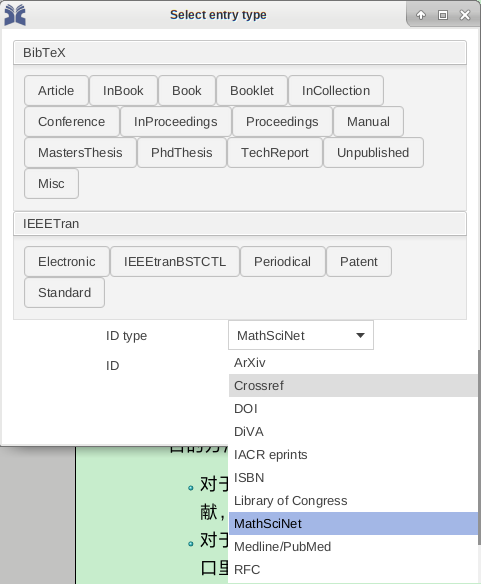
\includegraphics[width=0.618\textwidth]{pictures_01.png}
			\end{center}
			再点击
			\begin{center}
				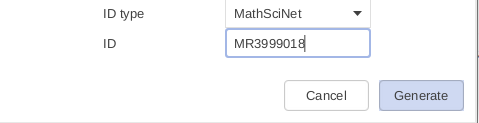
\includegraphics[width=0.618\textwidth]{pictures_02.png}
			\end{center}
			这样,就加入了,最终效果如图:
			\begin{center}
			
\includegraphics[width=0.618\textwidth]{pictures_03.png}
			\end{center}
		\item 第二类,手工添加引用信息到.bib文件。对于百度学术,选择引用,
			\begin{center}
			
\includegraphics[width=0.618\textwidth]{pictures_04.png}
			\end{center}
			选择 \BibTeX,
			\begin{center}
			
\includegraphics[width=0.618\textwidth]{pictures_05.png}
			\end{center}
			弹出来的窗口里全选复制
			\begin{center}
			
\includegraphics[width=0.618\textwidth]{pictures_06.png}
			\end{center}
			在JabRef主界面找到
			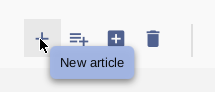
\includegraphics{pictures_20.png},
			点击添加一个article条目
			\begin{center}
			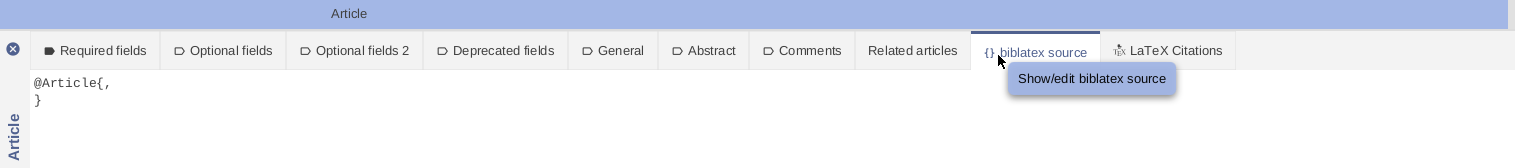
\includegraphics[width=0.618\textwidth]{pictures_21.png}
			\end{center}
			找到图中鼠标所指``\{\}Bib\LaTeX{} Source''位置,全选下方文本框中的内容,用之前已经复制好的内容替代,结果如下
			\begin{center}
			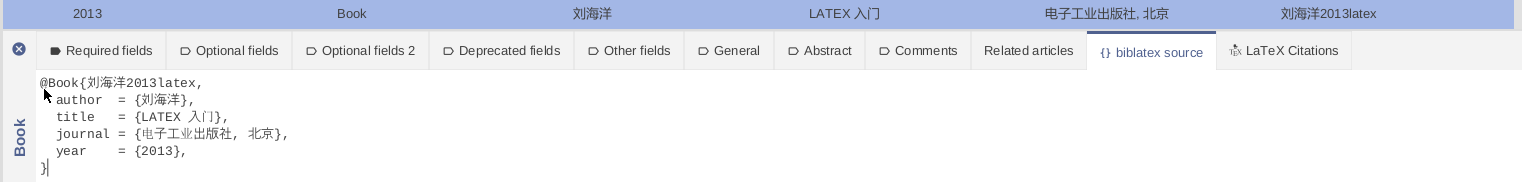
\includegraphics[width=0.618\textwidth]{pictures_22.png}
			\end{center}
			由于原来的引用内容有误,此处手工把article改成book类了。修改完毕,按Ctrl+S保存下bib库文件。
			\begin{note}
			也可以用文本编辑器打开.bib文件,粘贴到最后位置即可,注意保存一下。\\
			\end{note}
对于谷歌学术,选择逗号,
			\begin{center}
			
\includegraphics[width=0.618\textwidth]{pictures_07.png}
			\end{center}
			其余操作类似,最终是这样效果:
			\begin{center}
			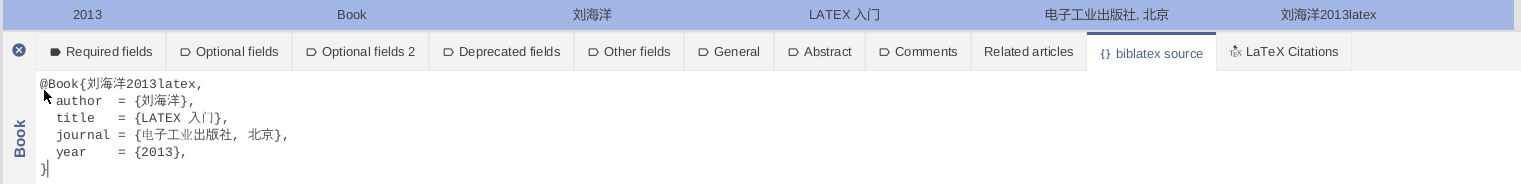
\includegraphics[width=0.618\textwidth]{pictures_23.png}
			\end{center}
	\end{itemize}
	\begin{note}
在Windows系统下,如果用文本编辑器打开.tex或者.bib文件是乱码,这是由于Windows创建的文本文件默认编码是ANSI,可以用“记事本”打开,“另存为”,编码格式选“utf8”,重新保存成utf8编码的文件即可。这样的操作也可以反过来,utf8编码的可以转成ANSI,适用于用传统编码的文本编辑器(如WinEdt)。
	\end{note}
\subsection{利用Zotero制作.bib文件}
Zotero的好处:
\begin{itemize}
	\item 是一个免费易用的Firefox扩展,它最大优点是结合浏览器实现对在线文献数据库网页中的文献题录直接抓取。
	\item 支持直接拖入pdf文件或者任意格式的附件,并自动提取pdf文档中的元数据生成文献条目信息。
	\item 支持标签分类,可以管理文献。
	\item 对中国知网等中文期刊支持很好,支持大陆版的DOI,ISBN等。
	\item 支持导入导出.bib文件。
\end{itemize}
		Zotero也支持多种方式添加文献条目,可以参考前面Jabref的添加操作,此处不再赘述。
\section{重点二:在\TeX 源文件中使用生成的参考文献列表}
首先,需要注意的是\textcolor{red}{.bib文件和.tex文件最好放在同一文件夹下}。如果不是,需要在源文件中指明具体的路径和文件名,不需要扩展名.bib。\par
其次,需要在\TeX 源文件末尾加入这样两行\footnote{其中第一行,有的模板中可能已经加上了,就不需要再加了,但第二行是必须的。}:
		\begin{lstlisting}
			\bibliographystyle{plain}
			\bibliography{bib文件名1,bib文件名2,...}
		\end{lstlisting}
			\begin{note}
				此处plain是参考文献列表格式,我国出版机构文后参考文献著录规则大部分采用的是国标\href{http://www.sac.gov.cn/SACSearch/outlinetemplet/gjbzcx.jsp}{GB/T 7714}\cite{gbt7714_2015},最新的是\href{http://www.scal.edu.cn/dxtsgxb/201906120155}{2015}年修订的\footnote{本文模板采用的文后参考文献著录规则就是GB/T 7714}。具体的格式要看您投稿的机构,一般都会提供相应格式的.bst配置文件。当然生猛的您可以自己手工修改相应的.bst文件,调整格式,见\href{https://blog.csdn.net/chikily_yongfeng/article/details/86553359}{\LaTeX 自定义参考文献格式(配置 bst)}\cite{noauthor_latex_nodate}。
			\end{note}
如果希望bib文件中所有文献都列出来,在这两句话前面再加一句话:
		\begin{lstlisting}
			\nocite{*}
		\end{lstlisting}
否则,只有前面引用的才会出现在生成的参考文献列表里。
\subsection{利用Jabref实现一键引用}
	Jabref中,插入引用标志到文中具体位置,按如下“三步走”:
		\begin{itemize}
			\item 第一步,先在文本编辑器比如\TeX studio中,打开要编辑的.tex文件,把光标定位在要插入引用文献标志的位置;
			\begin{center}
			
\includegraphics[width=0.618\textwidth]{pictures_12.png}
			\end{center}
		\item 第二步,在Jabref中打开.bib文件,选择要插入的参考文献条目,多选按住Ctrl键。
			\begin{center}
			
\includegraphics[width=0.618\textwidth]{pictures_13.png}
			\end{center}
		\item 第三步,点击工具条中的图标
\includegraphics{pictures_11.png},或者按Ctrl+L键。
			\begin{center}
			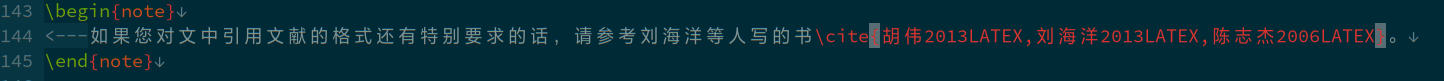
\includegraphics[width=0.618\textwidth]{pictures_14.png}
			\end{center}
		\end{itemize}
您会发现引用文献标志已经加到相应位置了,是不是很方便?有没有很惊喜?\\
如果您的Jabref工具栏中没有
\includegraphics{pictures_11.png},您需要在菜单栏选\\
``Options''$\to$``Preferences''$\to$``External programs'',\\
再从下拉菜单中选择您所用的文本编辑器,目前Jabref支持的编辑器有 \href{https://ftp.gnu.org/gnu/emacs/}{Emacs}, \href{https://www.lyx.org/}{Lyx}/\href{https://kile.sourceforge.io/}{Kile},\href{https://www.xm1math.net/texmaker/}{\TeX maker},\href{https://github.com/texstudio-org/texstudio/releases}{\TeX studio},\href{https://github.com/vim/vim/releases}{Vim},\href{http://www.winedt.com/}{WinEdt} 六种。
			\begin{center}
			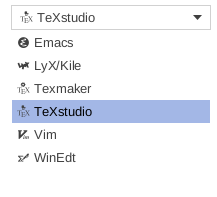
\includegraphics[width=0.618\textwidth]{pictures_10.png}
			\end{center}
\subsection{利用Zotero实现一键引用\cite{q_better_nodate}}
Zotero的一键引用需要在Zotero中安装\href{https://retorque.re/zotero-better-bibtex/}{Better \BibTeX{} for Zotero} 插件\footnote{您可以在\url{https://github.com/retorquere/zotero-better-bibtex/releases}处下载到最新的Better \BibTeX{} for Zotero插件,扩展名是.xpi。}。实现一键引用,需要如下三步:
\begin{itemize}
	\item 安装Better \BibTeX\\
		在Zotero的菜单中选择``Tools''$\to$ ``Add-ons'',再在弹出来的Add-ons Manager窗口中,右上角找到齿轮形状的``设置''按钮,鼠标左键单击,选择``Install Add-on From File...'',再找到刚下载的.xpi文件,按提示安装就可以了,中间可能需要重启Zotero两次。
	\item 设置导出Quick Copy的默认格式\\
		在Zotero的菜单中选择``Edit''$\to$ ``Preferences'',再在弹出来的 Zotero Preferences窗口中,找到``Export''项,有Quick Copy操作说明,在``Default Format''中找到``Better \BibTeX{} Citation Key Quick Copy'',选中即可。
	\item 一键引用\\
		最好先把光标定位在已经打开的编辑器中源文件的需要引用的位置,然后在Zotero中选中需要引用的参考文献条目,多选按住Ctrl键,在条目左边图标位置按住鼠标左键,直接拖到对应文本编辑器中需要引用的位置就可以了。
		\begin{note}
		对于\TeX studio编辑器,在选中文献条目上点击鼠标右键,会有``Push references to \TeX studio''选项,点击就可以添加到\TeX studio中的引用位置了。
			\begin{center}
			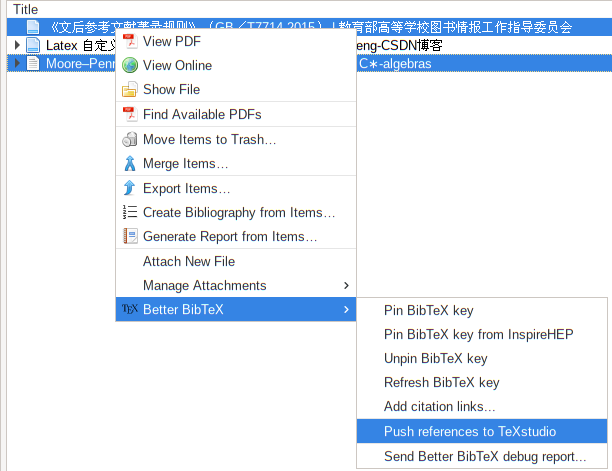
\includegraphics[width=0.618\textwidth]{pictures_19.png}
			\end{center}
		\end{note}
\end{itemize}
\subsection{手动引用参考文献}
	如果需要手工引用参考文献,直接复制对应文献条目的具体Bibtexkey值,
			\begin{center}
			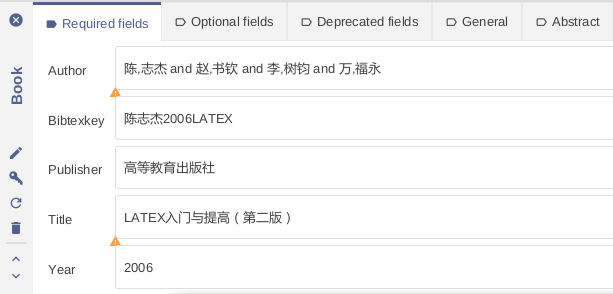
\includegraphics[width=0.618\textwidth]{pictures_15.png}
			\end{center}
			或者.bib文件中这个位置的字符串,下图中对应的红色部分的字符串:
			\begin{center}
			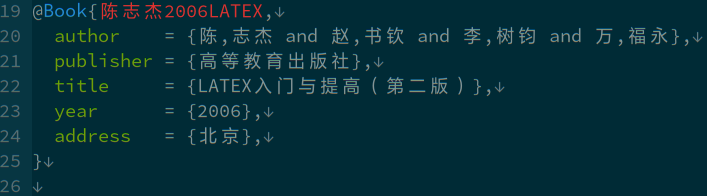
\includegraphics[width=0.618\textwidth]{pictures_16.png}
			\end{center}
	然后在源文件对应位置用如下命令即可:
	\begin{lstlisting}
	\cite{具体Bibtexkey值}
	\end{lstlisting}
\begin{note}
	如果您对文中引用文献的格式还有特别要求的话,请参考刘海洋等人写的书\cite{胡伟2013LATEX,刘海洋2013LATEX,陈志杰2006LATEX}。
\end{note}
\section{编译}
如果是\TeX studio编辑器的话,直接点
\includegraphics{pictures_17.png}(按F5效果同)或者
\includegraphics{pictures_18.png}(按F6效果同)就可以了。
如果您用的是别的编辑器(比如Vim,Emacs,WinEdit之类的),您需要执行如下四步\cite[第 380 页]{胡伟2013LATEX}:
\begin{itemize}
	\item 第一步:先编译.tex源文件一次,
	\item 第二步:用\BibTeX 编译.bib文件,参考命令:
		\begin{lstlisting}
		bibtex   具体bib文件名
		\end{lstlisting}
	\item 第三、四步:编译.tex文件\textcolor{red}{两}次,就可以正确生成引用位置了(否则引用位置有可能会出现问号,形如[?])。
\end{itemize}
\section{利益无关声明}
本文涉及到的程序,除了WinEdt是商业软件外,其余如\TeX 系统,Jabref和Zotero文献管理器,Vim,Emacs,\TeX studio等文本编辑器都是开源软件。本文也是以开源协议发布的,欢迎大家在开源协议下自由修改分享。本文链接:\url{https://github.com/zalois/note4JabrefandZotero}
\section{致谢}
感谢创建\TeX 的Donald Ervin Knuth先生,感谢Jabref和Zotero的贡献者们。
本文档套用的模板下载自\href{https://github.com/ElegantLaTeX/ElegantNote}{https://github.com/Elegant\LaTeX/ElegantNote},感谢模板作者邓东升。\footnote{插播一个小广告:本文档系统环境:\href{https://mirrors.slackware.com/slackware/slackware64-current/}{Slackware64-Current} + \href{https://www.tug.org/texlive/}{\TeX live 2020} + \href{https://www.vim.org/}{Vim 8.2.1456}}
%\nocite{*}
%\bibliographystyle{plain}
\bibliography{Jabref和Zotero使用笔记}
\end{document}
